\section{Pregunta N$^{\circ}$1\qquad Andre Gilmer Santos Felix}

\begin{frame}
    \begin{enumerate}\setcounter{enumi}{0}
        \item

              Calcule la curvatura de la gráfica del polinomio de
              $B_{5,3}$.
    \end{enumerate}

    \begin{solution}
        La gráfica de una función $y=f\left(x\right)$ es un caso
        especial de una curva parametrizada, de la forma

        \begin{equation*}
            \begin{cases}
                x & =t               \\
                y & =f\left(t\right)
            \end{cases}
        \end{equation*}

        la curvatura viene dada por

        \begin{equation*}
            \kappa=
            \dfrac{
                y^{\prime\prime}
            }{
                {\left(1+{y^{\prime}}^{2}\right)}^{\frac{3}{2}}
            }.
        \end{equation*}

        El polinomio de Bernstein $B_{n,k}$ es
        \begin{math}
            B_{n,k}\left(t\right)=
            \binom{n}{k}
            t^{k}
            \left(1-t\right)^{n-k}
        \end{math},
        $\forall t\in\left[0,1\right]$.
        Entonces,
        \begin{math}
            B_{5,3}\left(t\right)=
            \binom{5}{3}
            t^{3}
            \left(1-t\right)^{5-3}=
            10t^{3}{\left(1-t\right)}^{2}.
        \end{math}
        La segunda derivada de este polinomio es
    \end{solution}
\end{frame}

\begin{frame}
    \begin{solution}
        \begin{figure}[ht!]
            \centering
            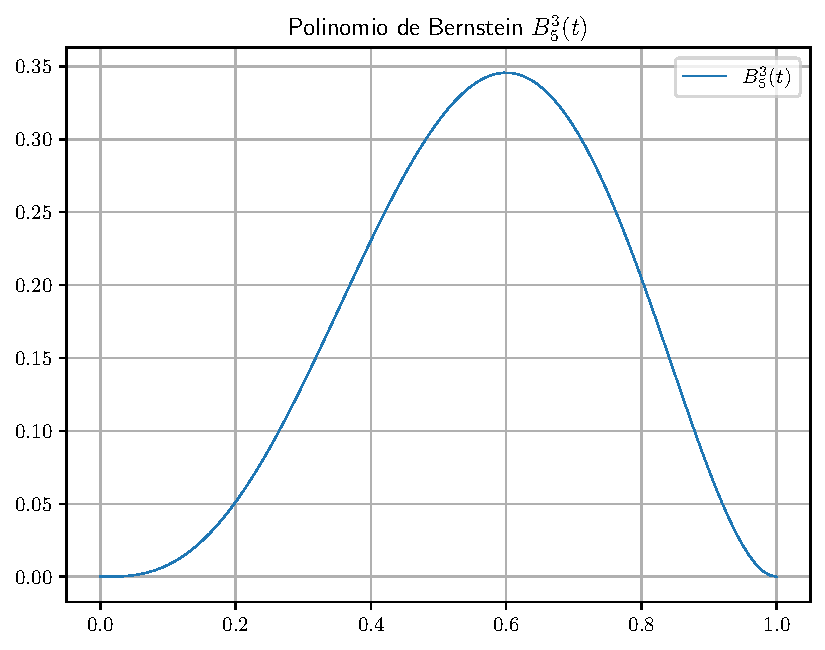
\includegraphics[width=.72\paperwidth]{p1}
        \end{figure}
    \end{solution}
\end{frame}